\documentclass[a4paper,12pt]{article} 
\usepackage{mathrsfs}
\usepackage[utf8]{inputenc}
\usepackage[spanish]{babel}
\usepackage{amsmath}
\usepackage{amsfonts}
\usepackage{amssymb} 
\usepackage{graphicx} 
\usepackage{hyperref} 
\usepackage{wrapfig}
\usepackage{enumitem}
\usepackage{fancyhdr}
\usepackage{float}
\usepackage{eurosym}
\usepackage{color}
\usepackage{circuitikz}
\usepackage{titling}
\usepackage{hyperref}
\usepackage{media9}
\usepackage{lipsum}
\usepackage{tocbibind}
\usepackage{listings}
\usepackage{tabularx}
\usepackage{tcolorbox}
\usepackage{bookmark}
\usepackage{media9}
\usepackage[table]{xcolor}
\definecolor{lightblue}{RGB}{228, 244, 253}
\usepackage{listings}
\usepackage{color}

\definecolor{dkgreen}{rgb}{0,0.6,0}
\definecolor{gray}{rgb}{0.5,0.5,0.5}
\definecolor{mauve}{rgb}{0.58,0,0.82}

\lstset{frame=tb,
  language=Python,
  inputencoding=utf8,
  extendedchars=true,
  aboveskip=3mm,
  belowskip=3mm,
  showstringspaces=false,
  columns=flexible,
  basicstyle={\small\ttfamily},
  numbers=none,
  numberstyle=\tiny\color{gray},
  keywordstyle=\color{blue},
  commentstyle=\color{dkgreen},
  stringstyle=\color{mauve},
  breaklines=true,
  breakatwhitespace=true,
  tabsize=3,
  literate=%
    {á}{{\'a}}1
    {é}{{\'e}}1
    {í}{{\'i}}1
    {ó}{{\'o}}1
    {ú}{{\'u}}1
    {ñ}{{\~n}}1
    {č}{{\v{c}}}1
}
\usepackage[left=3cm,right=3cm,top=3cm,bottom=4cm]{geometry}
\sloppy

\pagestyle{fancy}
\providecommand{\abs}[1]{\lvert#1\rvert}
\providecommand{\norm}[1]{\lVert#1\rVert}

%%% Para las cabeceras
\newcommand{\hsp}{\hspace{20pt}}
\newcommand{\HRule}{\rule{\linewidth}{0.5mm}}
\headheight=50pt
%%% 
\newcommand{\vacio}{\textcolor{white}{ .}}

%%% Para que las ecuaciones se numeren
%%% con el número de sección y el de ecuación.
\renewcommand{\theequation}{\thesection.\arabic{equation}}


% Color azul para algunos 
% textos de la portada
\definecolor{azulportada}{rgb}{0.16, 0.32, 0.75}

%%%% Azul para textos de headings
\definecolor{azulinterior}{rgb}{0.0, 0.2, 0.6}

%%%%%%%%%%%%%%%%%%%%%%%%%%%%%%%%
%%%%%% Datos del proyecto %%%%%%
%%%%%%%%%%%%%%%%%%%%%%%%%%%%%%%%
%%%TÍTULO
%%% Escribirlo en minúsculas, el programa
%%% lo pondrá en mayúsculas en la portada.

\title{Procesamiento de imágenes}

%%%% AUTORES
\author{Lydia Ruiz Martínez \and Pablo Tuñón Laguna}

%%%%%%%%%%%%%%%%%%%%%
%%%%%%%%%%%%%%%%%%%%
\begin{document}

%%%%%%%%%%%%%%%%%%%%%%%%%%%%%%%
%%%%%%%%%%%%%%%%%%%%%%%%%%%%%%%
\begin{titlepage} %%%%% Aquí no hay que tocar nada.
	%%%% Las siguientes instrucciones generarán automáticamente
	%%%% la portada de tu proyecto.
	%%% Cambio de la estructura de esta página
\newgeometry{left=0.6cm,top=1.3cm,bottom=1.2cm}

\fbox{\parbox[c]{18.5cm}{
\begin{center}
\vspace{1.5cm}
{\fontfamily{ptm}\fontsize{24}{28.8}\selectfont{Universidad Pontificia de Comillas}}\\
[3.5em]
{\fontfamily{ptm}\fontsize{24}{5}\selectfont{ICAI}}\\
[4.5em]
{\fontfamily{ptm}\fontsize{28}{5}\selectfont{LABORATORIO 2}}\\
[2cm]
{\fontfamily{ptm}\fontsize{24}{5}\selectfont{Visión por Ordenador I}}\\
[2cm]

% Autor del trabajo de investigación
\textcolor{azulportada}{\fontfamily{ptm}\fontsize{16}{5}\selectfont{\theauthor}}\\
[2cm]
% Título del trabajo
\textcolor{azulportada}
{\fontfamily{ptm}\fontsize{30}{5}\selectfont{\textsc{\thetitle}}}\\
%{\Huge\textbf{\thetitle}}\\
[1.2cm]

\includegraphics[width=10cm]{fonts/Logo ICAI.png}
\\[1.8cm]

{\fontfamily{ptm}\fontsize{16}{5}\selectfont{Curso 2024-2025}}\\
[4cm]
\end{center}
}}
\end{titlepage}
 
 \restoregeometry
 %%%% Volvemos a la estructura de la página normal

%%%%%%%%%%%%%%%%%%%%%%%%%%%%%%

{%\Large

%%%Encabezamiento y pie de página
%%% También se genera automáticamente
%%% Mejor no tocarlo mucho.
\renewcommand{\headrulewidth}{0.5pt}
\fancyhead[R]{
	\textcolor{azulinterior}{\fontfamily{ptm}\fontsize{14}{4}\selectfont{\textbf{\thetitle}}}\\
\textcolor{azulportada}{\fontfamily{ptm}\fontsize{10}{3}\selectfont{Laboratorio 2 de Visión por Ordenador I}}\\
{\fontfamily{ptm}\fontsize{10}{3}\selectfont{\theauthor}}}
\fancyhead[L]{\vacio}

\pagestyle{fancy}
\renewcommand{\footrulewidth}{0.5pt}
\fancyfoot[L]{\footnotesize Universidad Pontificia de Comillas (ICAI) --- curso 2024-2025}
\fancyfoot[C]{\vacio}
\fancyfoot[R]{\footnotesize Página \thepage}

%%%%%%%%%%%%%%%%%%%%
\newpage

\renewcommand{\contentsname}{Índice}
\addtocontents{toc}{\protect\setcounter{tocdepth}{-1}} % Quita el índice de la tabla de contenidos
\tableofcontents
\addtocontents{toc}{\protect\setcounter{tocdepth}{2}}

\newpage

\section{Introducción}

El procesamiento de imágenes es un área fundamental de la visión por ordenador que se enfoca en la manipulación y el análisis
de imágenes digitales. A diferencia de un ser humano, que puede interpretar imágenes de manera intuitiva, un ordenador necesita
algoritmos específicos que le permitan extraer información útil de las matrices de píxeles que componen cada imagen. Estos 
algoritmos permiten a los sistemas de visión por ordenador realizar tareas como la segmentación, la detección de bordes 
y la aplicación de filtros, convirtiendo datos visuales en información comprensible.

\vspace{0.5cm}
La segmentación de imágenes por color es una técnica crucial que permite identificar y aislar objetos de interés en una imagen 
basándose en sus características cromáticas. Este proceso es esencial en múltiples aplicaciones, desde la automatización 
industrial hasta la medicina, donde la identificación precisa de regiones de interés puede marcar la diferencia en el análisis
y la toma de decisiones. La capacidad de un ordenador para diferenciar colores y reconocer patrones en el espacio de color 
adecuado es un paso inicial vital en la interpretación de las imágenes.

\vspace{0.5cm}
Además, la aplicación de filtros es otra herramienta poderosa en el procesamiento de imágenes. Filtros como el gaussiano, 
Sobel y Canny se utilizan para suavizar imágenes, eliminar el ruido y detectar bordes, respectivamente. La detección de bordes
es especialmente relevante, ya que resalta las transiciones significativas en una imagen, facilitando la identificación de
  formas y estructuras. Al aplicar y comparar estos filtros, se pueden evaluar sus efectos en la calidad de la imagen y la
efectividad del análisis posterior.

\vspace{0.5cm}
Finalmente, el uso de operadores morfológicos complementa estas técnicas al permitir la manipulación de la estructura de los
objetos en las imágenes a nivel de píxel. Este enfoque es fundamental para mejorar los resultados de la segmentación y la 
detección, proporcionando una comprensión más profunda de las características presentes en las imágenes. En esta práctica, 
se implementarán estas técnicas utilizando Python y las librerías OpenCV e Imageio principalmente.

\newpage

\section{Segmentación por color}

La segmentación de imágenes por colores es una técnica sencilla y útil en aplicaciones en las que se tiene un gran control
sobre las condiciones de contorno: iluminación, tipo de objeto que se espera encontrar, colo de fondo, etc.
En esta práctica, se enfocará en la segmentación de los colores blancos
y naranjas en imágenes de peces. 

Para comenzar, se procede a cargar las imágenes desde la carpeta donde se almacenan los archivos de  las imágenes 
a procesar. Una vez cargadas, se implementan métodos para visualizar y guardar las imágenes, permitiendo 
una fácil manipulación y verificación de los resultados.

El siguiente paso consiste en cambiar el espacio de color de las imágenes de \textit{BGR} a \textit{HSV}, lo cual es esencial
para una mejor discriminación de los colores de interés. Este cambio de espacio de color transforma la representación de los 
colores, separando la crominancia de la intensidad, y facilita la identificación de los tonos deseados. Utilizando el método
\textit{cv2.cvtColor()} de OpenCV, se transformarán las imágenes para prepararlas para la segmentación. Este cambio es similar
a convertir un sistema de coordenadas cartesianas a uno polar, donde los colores se pueden manejar de manera más intuitiva.

Una vez que las imágenes estén en el espacio de color adecuado, se procede a generar máscaras para los colores naranjas y 
blancos, utilizando los métodos \textit{cv2.inRange()} y \textit{cv2.bitwise\_and()} de OpenCV. Estas máscaras permiten segmentar
las partes relevantes de las imágenes, destacando los píxeles de interés y eliminando aquellos que no corresponden. 

\begin{figure}[H]
  \centering
  \begin{minipage}[b]{0.45\textwidth}
      \centering
      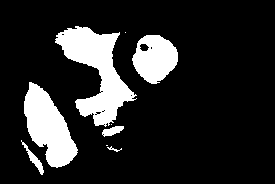
\includegraphics[width=\textwidth]{src/processed_data/orange_mask_0.png}
      \caption{Imagen 1 original, dataset.}
      \label{fig:izquierda1}
  \end{minipage}
  \hfill
  \begin{minipage}[b]{0.45\textwidth}
      \centering
      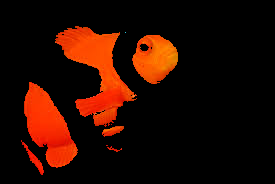
\includegraphics[width=\textwidth]{src/processed_data/orange_segmented_0.png}
      \caption{Imagen 1 corregida, autoría propia.}
      \label{fig:derecha1}
  \end{minipage}
  
  \vspace{1cm} 

  \begin{minipage}[b]{0.45\textwidth}
      \centering
      
\includegraphics[width=\textwidth]{src/processed_data/white_mask_0.png}
      \caption{Imagen 2 original, dataset.}
      \label{fig:izquierda2}
  \end{minipage}
  \hfill
  \begin{minipage}[b]{0.45\textwidth}
      \centering
      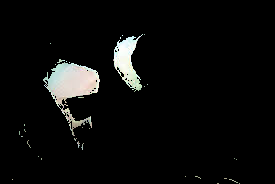
\includegraphics[width=\textwidth]{src/processed_data/white_segmented_0.png}
      \caption{Imagen 2 corregida, autoría propia.}
      \label{fig:derecha2}
  \end{minipage}
\end{figure}


\section{Filtro Gaussiano y Detección de bordes: Sobel y Canny}

\section{Operadores morfológicos}

En esta sección, se implementan los operadores morfológicos de dilatación y erosión
utilizando un kernel de \(3 \times 3\) con valores de \(255\) (blanco) como structuring element. 

Se define el método de binarización, el cual convierte una imagen a escala de grises a una imagen 
binaria utilizando un umbral de \(127\). Este método emplea la función \textit{cv2.threshold} de 
OpenCV para realizar la conversión.

Se implementa el método de dilatación, que consiste en ampliar las áreas blancas de la imagen binaria. 
Para ello, se utiliza un padding de la imagen original para mantener las dimensiones tras el procesamiento. 
En este método, se recorren todos los píxeles de la imagen, y se reemplaza cada píxel por el valor máximo 
de sus vecinos en el kernel.

Asimismo, se implementa el método de erosión, que reduce las áreas blancas de la imagen. Al igual que en 
la dilatación, se utiliza un padding para conservar las dimensiones. En este caso, cada píxel se reemplaza 
por el valor mínimo de sus vecinos en el kernel.

\begin{figure}[h!]
  \centering
  \begin{minipage}[b]{0.45\textwidth}
      \centering
      \includegraphics[width=\textwidth]{src/morphological_operators/custom_dilate_0.png}
      \caption{Ajuste fino de intersección de cuadrícula, autoría propia.}
      \label{fig:izquierda1}
  \end{minipage}
  \hfill
  \begin{minipage}[b]{0.45\textwidth}
      \centering
      \includegraphics[width=\textwidth]{src/morphological_operators/custom_erode_0.png}
      \caption{Ajuste fino de intersección de cuadrícula, autoría propia.}
      \label{fig:derecha1}
  \end{minipage}

\end{figure}

\end{document}



